%\begin{figure*}[h!]
%\begin{center}
%	 \hspace*{-1.5cm}
%    \begin{tabular}{  c | c | c  c  c  c  c c }
%        %\hline
%        &\large{\textsf{Mean + Flow}}   &\large{\textsf{t = 1 }} &\large{\textsf{t = 7 }}    &\large{\textsf{t = 13 }} &\large{\textsf{t = 19 }}  &\large{\textsf{t = 25 }}  &\large{\textsf{t = 30 }}     \\ \hline
%
%		&\vspace{-.15in}&\\
%        \multirow{1}{*}[.5in]{ \rotatebox[origin=t]{90}{\large{\textsf{Truth}} }}
%        &
%		{{\includegraphics[height=0.1\linewidth]{figures/starwarps_results/rotation30Jy2/gt/pavgimg.pdf}} } &
%        \includegraphics[height=0.1\linewidth]{figures/starwarps_results/rotation30Jy2/gt/frames/gt_0.pdf} &
%        \includegraphics[height=0.1\linewidth]{figures/starwarps_results/rotation30Jy2/gt/frames/gt_6.pdf} &
%        \includegraphics[height=0.1\linewidth]{figures/starwarps_results/rotation30Jy2/gt/frames/gt_12.pdf} &
%        \includegraphics[height=0.1\linewidth]{figures/starwarps_results/rotation30Jy2/gt/frames/gt_18.pdf} &
%        \includegraphics[height=0.1\linewidth]{figures/starwarps_results/rotation30Jy2/gt/frames/gt_24.pdf} &
%        \includegraphics[height=0.1\linewidth]{figures/starwarps_results/rotation30Jy2/gt/frames/gt_29.pdf} 
%         \\   \hline
%         %&\vspace{.0001in}& \\
%         \multicolumn{8}{c}{  \large{\textsf{EHT 2017 WITH CALIBRATED DATA}}  }
%         \\ \hline
%        &\vspace{-.15in}&\\
%        \multirow{1}{*}[.5in]{ \rotatebox[origin=t]{90}{\small{\textsf{No Flow}} }}
%        &
%        {{\includegraphics[height=0.1\linewidth]{figures/starwarps_results/rotation30Jy2/visibilities/nomotion/pavgimg.pdf}} } &
%        \includegraphics[height=0.1\linewidth]{figures/starwarps_results/rotation30Jy2/visibilities/nomotion/frames/mean_0.pdf} &
%        \includegraphics[height=0.1\linewidth]{figures/starwarps_results/rotation30Jy2/visibilities/nomotion/frames/mean_6.pdf} &
%        \includegraphics[height=0.1\linewidth]{figures/starwarps_results/rotation30Jy2/visibilities/nomotion/frames/mean_12.pdf} &
%        \includegraphics[height=0.1\linewidth]{figures/starwarps_results/rotation30Jy2/visibilities/nomotion/frames/mean_18.pdf} &
%        \includegraphics[height=0.1\linewidth]{figures/starwarps_results/rotation30Jy2/visibilities/nomotion/frames/mean_24.pdf} &
%        \includegraphics[height=0.1\linewidth]{figures/starwarps_results/rotation30Jy2/visibilities/nomotion/frames/mean_29.pdf} 
%        \\          
%        &\vspace{-.15in}&\\
%        \multirow{1}{*}[.5in]{ \rotatebox[origin=t]{90}{\small{\textsf{Flow}} }}
%        &
%        {{\includegraphics[height=0.1\linewidth]{figures/starwarps_results/rotation30Jy2/visibilities/best/flow_pavg_best.pdf}} } &
%        \includegraphics[height=0.1\linewidth]{figures/starwarps_results/rotation30Jy2/visibilities/best/frames/mean_0.pdf} &
%        \includegraphics[height=0.1\linewidth]{figures/starwarps_results/rotation30Jy2/visibilities/best/frames/mean_6.pdf} &
%        \includegraphics[height=0.1\linewidth]{figures/starwarps_results/rotation30Jy2/visibilities/best/frames/mean_12.pdf} &
%        \includegraphics[height=0.1\linewidth]{figures/starwarps_results/rotation30Jy2/visibilities/best/frames/mean_18.pdf} &
%        \includegraphics[height=0.1\linewidth]{figures/starwarps_results/rotation30Jy2/visibilities/best/frames/mean_24.pdf} &
%        \includegraphics[height=0.1\linewidth]{figures/starwarps_results/rotation30Jy2/visibilities/best/frames/mean_29.pdf}  
%		 \\ \hline  	
%		 %&\vspace{.0001in}& \\
%		 \multicolumn{8}{c}{  \large{\textsf{EHT 2017+ WITH UNCALIBRATED DATA }}  }
%		\\ \hline
%        &\vspace{-.15in}&\\
%        \multirow{1}{*}[.5in]{ \rotatebox[origin=t]{90}{\small{\textsf{No Flow}} }}
%        &
%        {{\includegraphics[height=0.1\linewidth]{figures/starwarps_results/rotation30Jy2/amp-bispectrum/nomotion/pavgimg.pdf}} } &
%        \includegraphics[height=0.1\linewidth]{figures/starwarps_results/rotation30Jy2/amp-bispectrum/nomotion/frames/mean_0.pdf} &
%        \includegraphics[height=0.1\linewidth]{figures/starwarps_results/rotation30Jy2/amp-bispectrum/nomotion/frames/mean_6.pdf} &
%        \includegraphics[height=0.1\linewidth]{figures/starwarps_results/rotation30Jy2/amp-bispectrum/nomotion/frames/mean_12.pdf} &
%        \includegraphics[height=0.1\linewidth]{figures/starwarps_results/rotation30Jy2/amp-bispectrum/nomotion/frames/mean_18.pdf} &
%        \includegraphics[height=0.1\linewidth]{figures/starwarps_results/rotation30Jy2/amp-bispectrum/nomotion/frames/mean_24.pdf} &
%        \includegraphics[height=0.1\linewidth]{figures/starwarps_results/rotation30Jy2/amp-bispectrum/nomotion/frames/mean_29.pdf} 
%        \\          
%        &\vspace{-.15in}&\\
%        \multirow{1}{*}[.5in]{ \rotatebox[origin=t]{90}{\small{\textsf{Flow 1}} }}
%        &
%        {{\includegraphics[height=0.1\linewidth]{figures/starwarps_results/rotation30Jy2/amp-bispectrum/best/flow_pavg_best.pdf}} } &
%        \includegraphics[height=0.1\linewidth]{figures/starwarps_results/rotation30Jy2/amp-bispectrum/best/frames/mean_0.pdf} &
%        \includegraphics[height=0.1\linewidth]{figures/starwarps_results/rotation30Jy2/amp-bispectrum/best/frames/mean_6.pdf} &
%        \includegraphics[height=0.1\linewidth]{figures/starwarps_results/rotation30Jy2/amp-bispectrum/best/frames/mean_12.pdf} &
%        \includegraphics[height=0.1\linewidth]{figures/starwarps_results/rotation30Jy2/amp-bispectrum/best/frames/mean_18.pdf} &
%        \includegraphics[height=0.1\linewidth]{figures/starwarps_results/rotation30Jy2/amp-bispectrum/best/frames/mean_24.pdf} &
%        \includegraphics[height=0.1\linewidth]{figures/starwarps_results/rotation30Jy2/amp-bispectrum/best/frames/mean_29.pdf}  
%        \\ 
%        &\vspace{-.15in}&\\
%        \multirow{1}{*}[.5in]{ \rotatebox[origin=t]{90}{\small{\textsf{Flow 2}} }}
%        &
%        {{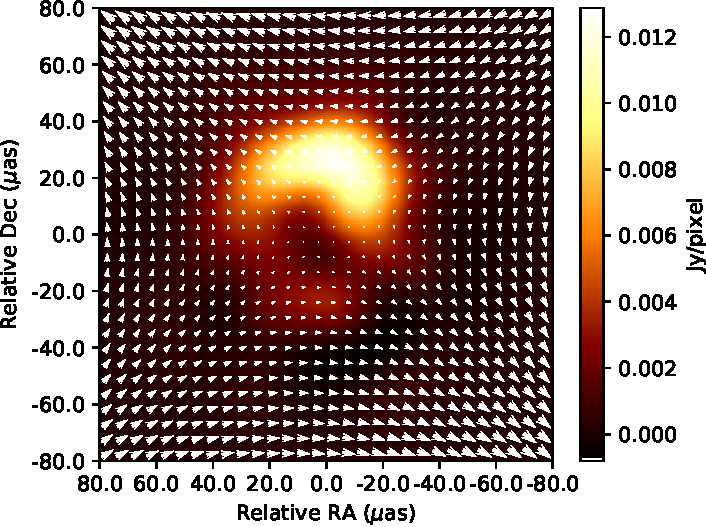
\includegraphics[height=0.1\linewidth]{figures/starwarps_results/rotation30/amp-bispectrum_sol2/best/flow_pavg_best.pdf}} } &
%        \includegraphics[height=0.1\linewidth]{figures/starwarps_results/rotation30/amp-bispectrum_sol2/best/frames/mean_0.pdf} &
%        \includegraphics[height=0.1\linewidth]{figures/starwarps_results/rotation30/amp-bispectrum_sol2/best/frames/mean_6.pdf} &
%        \includegraphics[height=0.1\linewidth]{figures/starwarps_results/rotation30/amp-bispectrum_sol2/best/frames/mean_12.pdf} &
%        \includegraphics[height=0.1\linewidth]{figures/starwarps_results/rotation30/amp-bispectrum_sol2/best/frames/mean_18.pdf} &
%        \includegraphics[height=0.1\linewidth]{figures/starwarps_results/rotation30/amp-bispectrum_sol2/best/frames/mean_24.pdf} &
%        \includegraphics[height=0.1\linewidth]{figures/starwarps_results/rotation30/amp-bispectrum_sol2/best/frames/mean_29.pdf}  
%        \\ \hline  	
%    \end{tabular}
%    \caption{\footnotesize{  }}
%\label{fig:rotation_example}
%\end{center}
%\end{figure*}







\begin{figure*}
	\begin{center}
		\setlength{\tabcolsep}{1pt}
		%\hspace*{-1.5cm}
		\begin{tabular}{  c | c | c  c  c  c  c c }
			
			
			%\hline
			\multirow{1}{*}[0.85in]{ \rotatebox[origin=t]{90}{\large{\textsf{uv-coverage}} }} &
			\includegraphics[height=0.12\linewidth]{figures/uvcoverage/uv_ehtfuture2_rotation30_small.pdf} 
			&
			\includegraphics[height=0.12\linewidth]{figures/uvcoverage/ehtfuture2_30/uv_ehtfuture2_rotation30_0.pdf} &
			\includegraphics[height=0.12\linewidth]{figures/uvcoverage/ehtfuture2_30/uv_ehtfuture2_rotation30_6.pdf} &
			\includegraphics[height=0.12\linewidth]{figures/uvcoverage/ehtfuture2_30/uv_ehtfuture2_rotation30_12.pdf} &
			\includegraphics[height=0.12\linewidth]{figures/uvcoverage/ehtfuture2_30/uv_ehtfuture2_rotation30_18.pdf} &
			\includegraphics[height=0.12\linewidth]{figures/uvcoverage/ehtfuture2_30/uv_ehtfuture2_rotation30_24.pdf} &
			\includegraphics[height=0.12\linewidth]{figures/uvcoverage/ehtfuture2_30/uv_ehtfuture2_rotation30_29.pdf} 
			\\  \hline
			&\vspace{-.1in} &&&&&&\\ 
			
			
			&\large{\textsf{Mean Frame}}   &\large{\textsf{GST = 17:00}} &\large{\textsf{19:30}}    &\large{\textsf{22:00}} &\large{\textsf{00:30}}  &\large{\textsf{03:00}}  &\large{\textsf{05:30}}     \\ \hline
			
			&\vspace{-.1in} &&&&&&\\
			\multirow{1}{*}[.5in]{ \rotatebox[origin=t]{90}{\large{\textsf{Truth}} }}
			&
			{{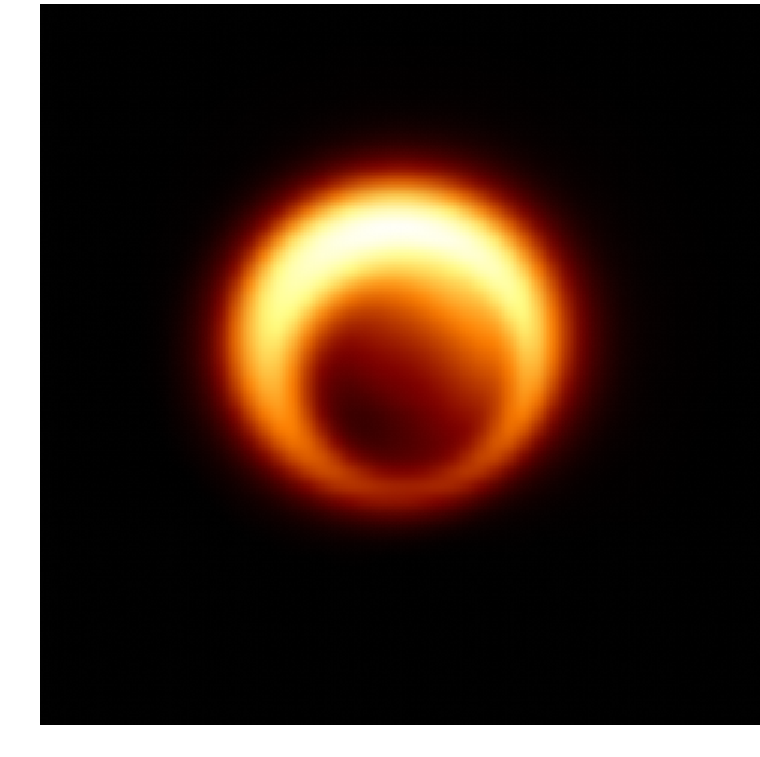
\includegraphics[height=0.12\linewidth]{figures/starwarps_results/rotation30/gt/pavgimg_noaxis.pdf}} } &
			\includegraphics[height=0.12\linewidth]{figures/starwarps_results/rotation30/gt/frames/gt_noaxis_0.pdf} &
			\includegraphics[height=0.12\linewidth]{figures/starwarps_results/rotation30/gt/frames/gt_noaxis_6.pdf} &
			\includegraphics[height=0.12\linewidth]{figures/starwarps_results/rotation30/gt/frames/gt_noaxis_12.pdf} &
			\includegraphics[height=0.12\linewidth]{figures/starwarps_results/rotation30/gt/frames/gt_noaxis_18.pdf} &
			\includegraphics[height=0.12\linewidth]{figures/starwarps_results/rotation30/gt/frames/gt_noaxis_24.pdf} &
			\includegraphics[height=0.12\linewidth]{figures/starwarps_results/rotation30/gt/frames/gt_noaxis_29.pdf} 
			\\   \hline
			&\vspace{-.1in} &&&&&&\\
			\multicolumn{8}{c}{  \large{\textsf{EHT2017+ WITH CALIBRATED DATA (VIS) }}  }
			\\ \hline
			&\vspace{-.1in} &&&&&&\\
			\multirow{1}{*}[.5in]{ \rotatebox[origin=t]{90}{\small{\textsf{Snapshot}} }}
			&
			{{\includegraphics[height=0.12\linewidth]{figures/starwarps_results/rotation30/rotation30_ehtfuture2_300_snapshot/Reconstructed_Average_Snapshot_vis.pdf}} } &
			\includegraphics[height=0.12\linewidth]{figures/starwarps_results/rotation30/rotation30_ehtfuture2_300_snapshot/Reconstructed_Snapshot_vis_0.pdf} &
			\includegraphics[height=0.12\linewidth]{figures/starwarps_results/rotation30/rotation30_ehtfuture2_300_snapshot/Reconstructed_Snapshot_vis_6.pdf} &
			\includegraphics[height=0.12\linewidth]{figures/starwarps_results/rotation30/rotation30_ehtfuture2_300_snapshot/Reconstructed_Snapshot_vis_12.pdf} &
			\includegraphics[height=0.12\linewidth]{figures/starwarps_results/rotation30/rotation30_ehtfuture2_300_snapshot/Reconstructed_Snapshot_vis_18.pdf} &
			\includegraphics[height=0.12\linewidth]{figures/starwarps_results/rotation30/rotation30_ehtfuture2_300_snapshot/Reconstructed_Snapshot_vis_24.pdf} &
			\includegraphics[height=0.12\linewidth]{figures/starwarps_results/rotation30/rotation30_ehtfuture2_300_snapshot/Reconstructed_Snapshot_vis_29.pdf} 
			\\          
			&\vspace{-.1in} &&&&&&\\
			\multirow{1}{*}[0.7in]{ \rotatebox[origin=t]{90}{  \specialcell{ \small{\textsf{StarWarps:}} \\  \small{\textsf{No Warp}}}  }}
			&
			{{\includegraphics[height=0.12\linewidth]{figures/starwarps_results/rotation30/visibilities/nomotion/pavgimg_noaxis.pdf}} } &
			\includegraphics[height=0.12\linewidth]{figures/starwarps_results/rotation30/visibilities/nomotion/frames/mean_noaxis_0.pdf} &
			\includegraphics[height=0.12\linewidth]{figures/starwarps_results/rotation30/visibilities/nomotion/frames/mean_noaxis_6.pdf} &
			\includegraphics[height=0.12\linewidth]{figures/starwarps_results/rotation30/visibilities/nomotion/frames/mean_noaxis_12.pdf} &
			\includegraphics[height=0.12\linewidth]{figures/starwarps_results/rotation30/visibilities/nomotion/frames/mean_noaxis_18.pdf} &
			\includegraphics[height=0.12\linewidth]{figures/starwarps_results/rotation30/visibilities/nomotion/frames/mean_noaxis_24.pdf} &
			\includegraphics[height=0.12\linewidth]{figures/starwarps_results/rotation30/visibilities/nomotion/frames/mean_noaxis_29.pdf} 
			\\          
			&\vspace{-.1in} &&&&&&\\
			\multirow{1}{*}[0.85in]{ \rotatebox[origin=t]{90}{  \specialcell{ \small{\textsf{StarWarps:}} \\  \small{\textsf{Infer Warp Field}}}  }}
			&
			{{\includegraphics[height=0.12\linewidth]{figures/starwarps_results/rotation30/visibilities/best/flow_pavg_best_noaxiscrop.pdf}} } &
			\includegraphics[height=0.12\linewidth]{figures/starwarps_results/rotation30/visibilities/best/frames/mean_noaxis_0.pdf} &
			\includegraphics[height=0.12\linewidth]{figures/starwarps_results/rotation30/visibilities/best/frames/mean_noaxis_6.pdf} &
			\includegraphics[height=0.12\linewidth]{figures/starwarps_results/rotation30/visibilities/best/frames/mean_noaxis_12.pdf} &
			\includegraphics[height=0.12\linewidth]{figures/starwarps_results/rotation30/visibilities/best/frames/mean_noaxis_18.pdf} &
			\includegraphics[height=0.12\linewidth]{figures/starwarps_results/rotation30/visibilities/best/frames/mean_noaxis_24.pdf} &
			\includegraphics[height=0.12\linewidth]{figures/starwarps_results/rotation30/visibilities/best/frames/mean_noaxis_29.pdf}  
			\\ \hline  	
			&\vspace{-.1in} &&&&&&\\
			\multicolumn{8}{c}{  \large{\textsf{EHT2017+ WITH ATMOSPHERIC PHASE ERROR (AMP \& BISP) }}  }
			\\ \hline
			&\vspace{-.1in} &&&&&&\\
			\multirow{1}{*}[.5in]{ \rotatebox[origin=t]{90}{\small{\textsf{Snapshot}} }}
			&
			{{\includegraphics[height=0.12\linewidth]{figures/starwarps_results/rotation30/rotation30_ehtfuture2_300_snapshot/Reconstructed_Average_Snapshot_AmpCphase.pdf}} } &
			\includegraphics[height=0.12\linewidth]{figures/starwarps_results/rotation30/rotation30_ehtfuture2_300_snapshot/Reconstructed_Snapshot_AmpCphase_0.pdf} &
			\includegraphics[height=0.12\linewidth]{figures/starwarps_results/rotation30/rotation30_ehtfuture2_300_snapshot/Reconstructed_Snapshot_AmpCphase_6.pdf} &
			\includegraphics[height=0.12\linewidth]{figures/starwarps_results/rotation30/rotation30_ehtfuture2_300_snapshot/Reconstructed_Snapshot_AmpCphase_12.pdf} &
			\includegraphics[height=0.12\linewidth]{figures/starwarps_results/rotation30/rotation30_ehtfuture2_300_snapshot/Reconstructed_Snapshot_AmpCphase_18.pdf} &
			\includegraphics[height=0.12\linewidth]{figures/starwarps_results/rotation30/rotation30_ehtfuture2_300_snapshot/Reconstructed_Snapshot_AmpCphase_24.pdf} &
			\includegraphics[height=0.12\linewidth]{figures/starwarps_results/rotation30/rotation30_ehtfuture2_300_snapshot/Reconstructed_Snapshot_AmpCphase_29.pdf} 
			\\          
			&\vspace{-.1in} &&&&&&\\
			\multirow{1}{*}[0.7in]{ \rotatebox[origin=t]{90}{  \specialcell{ \small{\textsf{StarWarps:}} \\  \small{\textsf{No Warp}}}  }}
			&
			{{\includegraphics[height=0.12\linewidth]{figures/starwarps_results/rotation30/amp-bispectrum_sol1/nomotion/pavgimg_noaxis.pdf}} } &
			\includegraphics[height=0.12\linewidth]{figures/starwarps_results/rotation30/amp-bispectrum_sol1/nomotion/frames/mean_noaxis_0.pdf} &
			\includegraphics[height=0.12\linewidth]{figures/starwarps_results/rotation30/amp-bispectrum_sol1/nomotion/frames/mean_noaxis_6.pdf} &
			\includegraphics[height=0.12\linewidth]{figures/starwarps_results/rotation30/amp-bispectrum_sol1/nomotion/frames/mean_noaxis_12.pdf} &
			\includegraphics[height=0.12\linewidth]{figures/starwarps_results/rotation30/amp-bispectrum_sol1/nomotion/frames/mean_noaxis_18.pdf} &
			\includegraphics[height=0.12\linewidth]{figures/starwarps_results/rotation30/amp-bispectrum_sol1/nomotion/frames/mean_noaxis_24.pdf} &
			\includegraphics[height=0.12\linewidth]{figures/starwarps_results/rotation30/amp-bispectrum_sol1/nomotion/frames/mean_noaxis_29.pdf} 
			\\          
			&\vspace{-.1in} &&&&&&\\
			\multirow{1}{*}[0.85in]{ \rotatebox[origin=t]{90}{  \specialcell{ \small{\textsf{StarWarps:}} \\  \small{\textsf{Infer Warp Field}}}  }}
			&
			{{\includegraphics[height=0.12\linewidth]{figures/starwarps_results/rotation30/amp-bispectrum_sol1/best/flow_pavg_best_noaxiscrop.pdf}} } &
			\includegraphics[height=0.12\linewidth]{figures/starwarps_results/rotation30/amp-bispectrum_sol1/best/frames/mean_noaxis_0.pdf} &
			\includegraphics[height=0.12\linewidth]{figures/starwarps_results/rotation30/amp-bispectrum_sol1/best/frames/mean_noaxis_6.pdf} &
			\includegraphics[height=0.12\linewidth]{figures/starwarps_results/rotation30/amp-bispectrum_sol1/best/frames/mean_noaxis_12.pdf} &
			\includegraphics[height=0.12\linewidth]{figures/starwarps_results/rotation30/amp-bispectrum_sol1/best/frames/mean_noaxis_18.pdf} &
			\includegraphics[height=0.12\linewidth]{figures/starwarps_results/rotation30/amp-bispectrum_sol1/best/frames/mean_noaxis_24.pdf} &
			\includegraphics[height=0.12\linewidth]{figures/starwarps_results/rotation30/amp-bispectrum_sol1/best/frames/mean_noaxis_29.pdf}  
			%			\\ 
			%			&\vspace{-.1in} &&&&&&\\
			%			\multirow{1}{*}[.5in]{ \rotatebox[origin=t]{90}{\small{\textsf{Flow 2}} }}
			%			&
			%			{{\includegraphics[height=0.12\linewidth]{figures/starwarps_results/rotation30/amp-bispectrum_sol2/best/flow_pavg_best.pdf}} } &
			%			\includegraphics[height=0.12\linewidth]{figures/starwarps_results/rotation30/amp-bispectrum_sol2/best/frames/mean_noaxis_0.pdf} &
			%			\includegraphics[height=0.12\linewidth]{figures/starwarps_results/rotation30/amp-bispectrum_sol2/best/frames/mean_noaxis_6.pdf} &
			%			\includegraphics[height=0.12\linewidth]{figures/starwarps_results/rotation30/amp-bispectrum_sol2/best/frames/mean_noaxis_12.pdf} &
			%			\includegraphics[height=0.12\linewidth]{figures/starwarps_results/rotation30/amp-bispectrum_sol2/best/frames/mean_noaxis_18.pdf} &
			%			\includegraphics[height=0.12\linewidth]{figures/starwarps_results/rotation30/amp-bispectrum_sol2/best/frames/mean_noaxis_24.pdf} &
			%			\includegraphics[height=0.12\linewidth]{figures/starwarps_results/rotation30/amp-bispectrum_sol2/best/frames/mean_noaxis_29.pdf}  
			\\ \hline  	
		\end{tabular}
		\caption{{\bf Time-resolved reconstruction of Video 1:} Video 1 contains an image rotating clockwise by $180^{\circ}$ over the course of the observation. At each time, the interferometric telescope array measures values related to 2D spatial frequencies of the current underlying image, shown in the row labeled `Truth'. These are indicated by the dots on the uv-coverage plots. As light emitted from the source is real-valued we obtain two values on opposite sides of the frequency plane -- each independent set of measurements displayed as either black or red. We present results obtained when using data with no atmospheric error (VIS) as well as when there is atmospheric phase error and we must use data products invariant to its effects (AMP \& BISP).
			Below the true images, we show a subset of images from the baseline 'snapshot imaging' method and compare it to our StarWarps reconstructed video obtained when we assume a static warp field or an inferred warp field. The mean image for each sequence is shown in the leftmost column. In the case that we simultaneously estimate a warp field, we indicate the resulting field as arrows on the mean image. Our method substantially improves results over the snapshot method, especially in the case of atmospheric error when the absolute position of the source cannot be recovered. Additionally, our proposed method can estimate a warp field that gives a sense of the underlying motion of the emission region. This can help to improve results, most notably for the calibrated data (VIS). }
		\label{fig:rotation_example1}
	\end{center}
\end{figure*}





















\begin{figure*}
	\begin{center}
		\setlength{\tabcolsep}{1pt}
		%\hspace*{-1.5cm}
		\begin{tabular}{  c | c | c  c  c  c  c c }
			%\hline
			
			\multirow{1}{*}[0.85in]{ \rotatebox[origin=t]{90}{\large{\textsf{uv-coverage}} }}
			&
			\includegraphics[height=0.12\linewidth]{figures/uvcoverage/uv_ehtfuture2_small.pdf} 
			&
			\includegraphics[height=0.12\linewidth]{figures/uvcoverage/ehtfuture2_173/uv_ehtfuture2_\HSa.pdf} &
			\includegraphics[height=0.12\linewidth]{figures/uvcoverage/ehtfuture2_173/uv_ehtfuture2_\HSb.pdf} &
			\includegraphics[height=0.12\linewidth]{figures/uvcoverage/ehtfuture2_173/uv_ehtfuture2_\HSc.pdf} &
			\includegraphics[height=0.12\linewidth]{figures/uvcoverage/ehtfuture2_173/uv_ehtfuture2_\HSd.pdf} &
			\includegraphics[height=0.12\linewidth]{figures/uvcoverage/ehtfuture2_173/uv_ehtfuture2_\HSe.pdf} &
			\includegraphics[height=0.12\linewidth]{figures/uvcoverage/ehtfuture2_173/uv_ehtfuture2_\HSf.pdf} 
			\\   \hline
			&\vspace{-.1in} &&&&&&\\
			
			&\large{\textsf{Mean Frame}}   &\large{\textsf{GST = 20:10 }} &\large{\textsf{20:20 }}    &\large{\textsf{20:30 }} &\large{\textsf{20:40 }}  &\large{\textsf{20:50 }}  &\large{\textsf{21:00 }}     \\ \hline
			
			&\vspace{-.1in} &&&&&&\\
			\multirow{1}{*}[.5in]{ \rotatebox[origin=t]{90}{\large{\textsf{Truth}} }}
			&
			{{\includegraphics[height=0.12\linewidth]{figures/starwarps_results/hotspot100sR2/gt/pavgimg_noaxis.pdf}} } &
			\includegraphics[height=0.12\linewidth]{figures/starwarps_results/hotspot100sR2/gt/frames/gt_noaxis_\HSa.pdf} &
			\includegraphics[height=0.12\linewidth]{figures/starwarps_results/hotspot100sR2/gt/frames/gt_noaxis_\HSb.pdf} &
			\includegraphics[height=0.12\linewidth]{figures/starwarps_results/hotspot100sR2/gt/frames/gt_noaxis_\HSc.pdf} &
			\includegraphics[height=0.12\linewidth]{figures/starwarps_results/hotspot100sR2/gt/frames/gt_noaxis_\HSd.pdf} &
			\includegraphics[height=0.12\linewidth]{figures/starwarps_results/hotspot100sR2/gt/frames/gt_noaxis_\HSe.pdf} &
			\includegraphics[height=0.12\linewidth]{figures/starwarps_results/hotspot100sR2/gt/frames/gt_noaxis_\HSf.pdf} 
			\\   \hline
			&\vspace{-.1in} &&&&&&\\
			\multicolumn{8}{c}{  \large{\textsf{EHT2017+ WITH CALIBRATED DATA (VIS) }}  }
			\\ \hline
			&\vspace{-.1in} &&&&&&\\
			\multirow{1}{*}[.5in]{ \rotatebox[origin=t]{90}{\small{\textsf{Snapshot}} }}
			&
			{{\includegraphics[height=0.12\linewidth]{figures/starwarps_results/hotspot100sR2/hotspot100sR2_ehtfuture2_100_snapshot/Reconstructed_Average_Snapshot_vis.pdf}} } &
			\includegraphics[height=0.12\linewidth]{figures/starwarps_results/hotspot100sR2/hotspot100sR2_ehtfuture2_100_snapshot/Reconstructed_Snapshot_vis_\HSa.pdf} &
			\includegraphics[height=0.12\linewidth]{figures/starwarps_results/hotspot100sR2/hotspot100sR2_ehtfuture2_100_snapshot/Reconstructed_Snapshot_vis_\HSb.pdf} &
			\includegraphics[height=0.12\linewidth]{figures/starwarps_results/hotspot100sR2/hotspot100sR2_ehtfuture2_100_snapshot/Reconstructed_Snapshot_vis_\HSc.pdf} &
			\includegraphics[height=0.12\linewidth]{figures/starwarps_results/hotspot100sR2/hotspot100sR2_ehtfuture2_100_snapshot/Reconstructed_Snapshot_vis_\HSd.pdf} &
			\includegraphics[height=0.12\linewidth]{figures/starwarps_results/hotspot100sR2/hotspot100sR2_ehtfuture2_100_snapshot/Reconstructed_Snapshot_vis_\HSe.pdf} &
			\includegraphics[height=0.12\linewidth]{figures/starwarps_results/hotspot100sR2/hotspot100sR2_ehtfuture2_100_snapshot/Reconstructed_Snapshot_vis_\HSf.pdf} 
			\\          
			&\vspace{-.1in} &&&&&&\\
			\multirow{1}{*}[0.7in]{ \rotatebox[origin=t]{90}{  \specialcell{ \small{\textsf{StarWarps:}} \\  \small{\textsf{No Warp}}}  }}
			&
			{{\includegraphics[height=0.12\linewidth]{figures/starwarps_results/hotspot100sR2/ehtfuture2_100_visibility/nomotion/pavgimg_noaxis.pdf}} } &
			\includegraphics[height=0.12\linewidth]{figures/starwarps_results/hotspot100sR2/ehtfuture2_100_visibility/nomotion/frames/mean_noaxis_\HSa.pdf} &
			\includegraphics[height=0.12\linewidth]{figures/starwarps_results/hotspot100sR2/ehtfuture2_100_visibility/nomotion/frames/mean_noaxis_\HSb.pdf} &
			\includegraphics[height=0.12\linewidth]{figures/starwarps_results/hotspot100sR2/ehtfuture2_100_visibility/nomotion/frames/mean_noaxis_\HSc.pdf} &
			\includegraphics[height=0.12\linewidth]{figures/starwarps_results/hotspot100sR2/ehtfuture2_100_visibility/nomotion/frames/mean_noaxis_\HSd.pdf} &
			\includegraphics[height=0.12\linewidth]{figures/starwarps_results/hotspot100sR2/ehtfuture2_100_visibility/nomotion/frames/mean_noaxis_\HSe.pdf} &
			\includegraphics[height=0.12\linewidth]{figures/starwarps_results/hotspot100sR2/ehtfuture2_100_visibility/nomotion/frames/mean_noaxis_\HSf.pdf} 
			\\          
			&\vspace{-.1in} &&&&&&\\
			\multirow{1}{*}[0.85in]{ \rotatebox[origin=t]{90}{  \specialcell{ \small{\textsf{StarWarps:}} \\  \small{\textsf{Infer Warp Field}}}  }}
			&
			{{\includegraphics[height=0.12\linewidth]{figures/starwarps_results/hotspot100sR2/ehtfuture2_100_visibility/best/flow_pavg_best_noaxis.pdf}} } &
			\includegraphics[height=0.12\linewidth]{figures/starwarps_results/hotspot100sR2/ehtfuture2_100_visibility/best/frames/mean_noaxis_\HSa.pdf} &
			\includegraphics[height=0.12\linewidth]{figures/starwarps_results/hotspot100sR2/ehtfuture2_100_visibility/best/frames/mean_noaxis_\HSb.pdf} &
			\includegraphics[height=0.12\linewidth]{figures/starwarps_results/hotspot100sR2/ehtfuture2_100_visibility/best/frames/mean_noaxis_\HSc.pdf} &
			\includegraphics[height=0.12\linewidth]{figures/starwarps_results/hotspot100sR2/ehtfuture2_100_visibility/best/frames/mean_noaxis_\HSd.pdf} &
			\includegraphics[height=0.12\linewidth]{figures/starwarps_results/hotspot100sR2/ehtfuture2_100_visibility/best/frames/mean_noaxis_\HSe.pdf} &
			\includegraphics[height=0.12\linewidth]{figures/starwarps_results/hotspot100sR2/ehtfuture2_100_visibility/best/frames/mean_noaxis_\HSf.pdf} 
			\\ \hline  	
			&\vspace{-.1in} &&&&&&\\
			\multicolumn{8}{c}{  \large{\textsf{EHT2017+ WITH ATMOSPHERIC PHASE ERROR (AMP \& BISP) }}  }
			\\ \hline
			&\vspace{-.1in} &&&&&&\\
			\multirow{1}{*}[.5in]{ \rotatebox[origin=t]{90}{\small{\textsf{Snapshot}} }}
			&
			{{\includegraphics[height=0.12\linewidth]{figures/starwarps_results/hotspot100sR2/hotspot100sR2_ehtfuture2_100_snapshot/Reconstructed_Average_Snapshot_AmpCphase.pdf}} } &
			\includegraphics[height=0.12\linewidth]{figures/starwarps_results/hotspot100sR2/hotspot100sR2_ehtfuture2_100_snapshot/Reconstructed_Snapshot_AmpCphase_\HSa.pdf} &
			\includegraphics[height=0.12\linewidth]{figures/starwarps_results/hotspot100sR2/hotspot100sR2_ehtfuture2_100_snapshot/Reconstructed_Snapshot_AmpCphase_\HSb.pdf} &
			\includegraphics[height=0.12\linewidth]{figures/starwarps_results/hotspot100sR2/hotspot100sR2_ehtfuture2_100_snapshot/Reconstructed_Snapshot_AmpCphase_\HSc.pdf} &
			\includegraphics[height=0.12\linewidth]{figures/starwarps_results/hotspot100sR2/hotspot100sR2_ehtfuture2_100_snapshot/Reconstructed_Snapshot_AmpCphase_\HSd.pdf} &
			\includegraphics[height=0.12\linewidth]{figures/starwarps_results/hotspot100sR2/hotspot100sR2_ehtfuture2_100_snapshot/Reconstructed_Snapshot_AmpCphase_\HSe.pdf} &
			\includegraphics[height=0.12\linewidth]{figures/starwarps_results/hotspot100sR2/hotspot100sR2_ehtfuture2_100_snapshot/Reconstructed_Snapshot_AmpCphase_\HSf.pdf}  \\
			&\vspace{-.1in} &&&&&&\\
			\multirow{1}{*}[0.7in]{ \rotatebox[origin=t]{90}{  \specialcell{ \small{\textsf{StarWarps:}} \\  \small{\textsf{No Warp}}}  }}
			&
			{{\includegraphics[height=0.12\linewidth]{figures/starwarps_results/hotspot100sR2/ehtfuture2_100_amp-bispectrum/nomotion/pavgimg_noaxis.pdf}} } &
			\includegraphics[height=0.12\linewidth]{figures/starwarps_results/hotspot100sR2/ehtfuture2_100_amp-bispectrum/nomotion/frames/mean_noaxis_\HSa.pdf} &
			\includegraphics[height=0.12\linewidth]{figures/starwarps_results/hotspot100sR2/ehtfuture2_100_amp-bispectrum/nomotion/frames/mean_noaxis_\HSb.pdf} &
			\includegraphics[height=0.12\linewidth]{figures/starwarps_results/hotspot100sR2/ehtfuture2_100_amp-bispectrum/nomotion/frames/mean_noaxis_\HSc.pdf} &
			\includegraphics[height=0.12\linewidth]{figures/starwarps_results/hotspot100sR2/ehtfuture2_100_amp-bispectrum/nomotion/frames/mean_noaxis_\HSd.pdf} &
			\includegraphics[height=0.12\linewidth]{figures/starwarps_results/hotspot100sR2/ehtfuture2_100_amp-bispectrum/nomotion/frames/mean_noaxis_\HSe.pdf} &
			\includegraphics[height=0.12\linewidth]{figures/starwarps_results/hotspot100sR2/ehtfuture2_100_amp-bispectrum/nomotion/frames/mean_noaxis_\HSf.pdf} 
			\\          
			&\vspace{-.1in} &&&&&&\\
			\multirow{1}{*}[0.85in]{ \rotatebox[origin=t]{90}{  \specialcell{ \small{\textsf{StarWarps:}} \\  \small{\textsf{Infer Warp Field}}}  }}
			&
			{{\includegraphics[height=0.12\linewidth]{figures/starwarps_results/hotspot100sR2/ehtfuture2_100_amp-bispectrum/best/flow_pavg_best_noaxis.pdf}} } &
			\includegraphics[height=0.12\linewidth]{figures/starwarps_results/hotspot100sR2/ehtfuture2_100_amp-bispectrum/best/frames/mean_noaxis_49.pdf} &
			\includegraphics[height=0.12\linewidth]{figures/starwarps_results/hotspot100sR2/ehtfuture2_100_amp-bispectrum/best/frames/mean_noaxis_59.pdf} &
			\includegraphics[height=0.12\linewidth]{figures/starwarps_results/hotspot100sR2/ehtfuture2_100_amp-bispectrum/best/frames/mean_noaxis_69.pdf} &
			\includegraphics[height=0.12\linewidth]{figures/starwarps_results/hotspot100sR2/ehtfuture2_100_amp-bispectrum/best/frames/mean_noaxis_79.pdf} &
			\includegraphics[height=0.12\linewidth]{figures/starwarps_results/hotspot100sR2/ehtfuture2_100_amp-bispectrum/best/frames/mean_noaxis_89.pdf} &
			\includegraphics[height=0.12\linewidth]{figures/starwarps_results/hotspot100sR2/ehtfuture2_100_amp-bispectrum/best/frames/mean_noaxis_90.pdf}  
			\\ \hline  	
		\end{tabular}
		\caption{{\bf Time-resolved reconstruction of Video 2:} Video 2 contains a sequence of a hotspot orbiting counter-clockwise around a black hole. We present time-resolved results obtained using data derived from this sequence. 
			Below the true images, we show a subset of images from the baseline 'snapshot imaging' method and compare it to our StarWarps reconstructed video obtained assuming a static warp field or an inferred warp field. The mean image for each sequence is shown in the leftmost column. If we simultaneously estimate a warp field, we indicate the resulting field as arrows on the mean image. 
			Our method substantially improve results over the snapshot method, especially in the case of atmospheric error when the absolute position of the source cannot be recovered. 
			Additionally, despite the fact that this hotspot video does not match our assumed motion model, using our proposed approach we were able to estimate a warp field that provides the direction of the source's true underlying motion. See the caption of Figure~\ref{fig:rotation_example1} for more detail. }
		\label{fig:rotation_example2}
	\end{center}
\end{figure*}


